\documentclass{article}
\usepackage{amsmath}
\usepackage[colorlinks=true]{hyperref}
\usepackage{color}
\usepackage{colortbl}
\usepackage{tikz}
\usetikzlibrary{patterns,matrix}
\usetikzlibrary{shapes,backgrounds}

\begin{document}

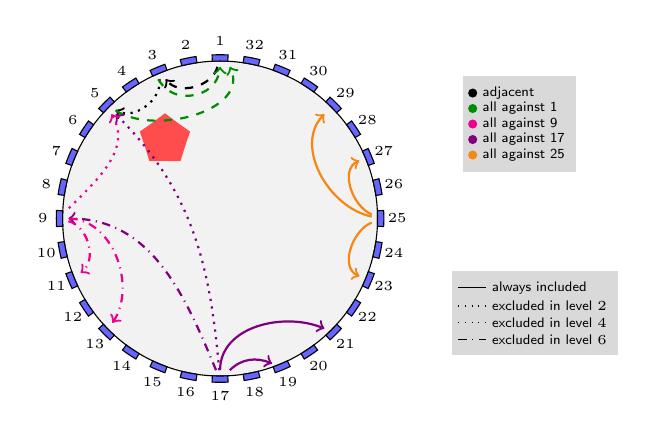
\begin{tikzpicture}
    \def\n{32} % Number of nodes
    \def\radius{2cm} % Radius of the circle
    \def\biggerradius{2.08cm}
    \def\smallradius{0.05cm} % Width of each node
    \draw[fill=gray!10] (0,0) circle (\radius);
    \node[star, star points=5, star point ratio=1.25, fill=red!70, inner sep=0.19cm] at (-0.7,1.0) {};
    \foreach \i in {1,...,\n}
    {
         \filldraw[fill=blue!60,opacity=1.0] ({-2.8125+(\i-1)*11.25}:\radius) arc ({-2.8125+(\i-1)*11.25}:{2.8125+(\i-1)*11.25}:\radius) -- ({2.8125+(\i-1)*11.25}:\biggerradius) arc ({2.8125+(\i-1)*11.25}:{-2.8125+(\i-1)*11.25}:\biggerradius) -- cycle;
        \node at ({360/\n * (\i-1)+90}:\radius+0.25cm) {\tiny{\i}};
        \node (\i) at ({360/\n * (\i-1)+90}:{\radius+0.05cm}) {};
    }
        \draw[dashed, ->, thick] (1) to [out={75+180},in={127.5+180}] (3);
        \draw[dotted, ->, thick] (3) to [out={97.5+180},in={150+180}] (5);

        \draw[dashed, ->, green!55!black, thick] plot [smooth, tension=1.5] coordinates { (3.south) (-0.328408, 1.56783) (1.south)};
        \draw[dashed, ->, green!55!black, thick] (5) to [out={180-212.5},in={115+180}] (1.south east);

        \draw[->, yellow!50!red, thick] (25) to [out={180+22.5},in={180-22.5}] (23);
        \draw[->, yellow!50!red, thick] (25) to [out={180-22.5},in={180+22.5}] (27);
        \draw[->, yellow!50!red, thick] (25) to [out={180-11.25},in={180+45.}] (29);

        \draw[->, blue!50!red, thick] (17) to [out={180-135},in={180-22.5}] (19);
        \draw[<-, blue!50!red, thick] (21) to [out={180-22.5},in={180+270}] (17);
        \draw[dashdotted, ->, blue!50!red, thick] (17) to [out={180-90+22.5},in={0}] (9);
        \draw[dotted, ->, blue!50!red, thick] (17) to [out={180-90+5},in={-45}] (5.south east);

        \draw[dotted, <-, magenta, thick] (5) to [out={180+165-45},in={180+180+45}] (9);
        \draw[dashdotted, ->, magenta, thick] (9) to [out={180+165},in={180+217.5}] (11);
        \draw[dashdotted, <-, magenta, thick] (13) to [out={180-123.5},in={180+180}] (9);
        \matrix[fill=gray!30, row sep=-1mm, inner sep=2pt, column 1/.style={anchor=base west}, column 2/.style={anchor=west}] at (3.8,1.2) {
          \node [draw, shape = circle, fill = black, minimum size = 0.1cm, inner sep=0pt] (){}; & \node[black,font=\tiny] {\textsf{adjacent}}; \\
          \node [draw=green!55!black, shape = circle, fill = green!55!black, minimum size = 0.1cm, inner sep=0pt] (){}; & \node[black,font=\tiny] {\textsf{all against 1}}; \\
          \node [draw=magenta, shape = circle, fill = magenta, minimum size = 0.1cm, inner sep=0pt] (){}; & \node[black,font=\tiny] {\textsf{all against 9}}; \\
          \node [draw=blue!50!red, shape = circle, fill = blue!50!red, minimum size = 0.1cm, inner sep=0pt] (){}; & \node[black,font=\tiny] {\textsf{all against 17}}; \\
          \node [draw=yellow!50!red, shape = circle, fill = yellow!50!red, minimum size = 0.1cm, inner sep=0pt] (){}; & \node[black,font=\tiny] {\textsf{all against 25}}; \\
        };
        \matrix[fill=gray!30, row sep=-0.5mm, inner sep=2pt, column 1/.style={anchor=base west}, column 2/.style={anchor=west}] at (4.0,-1.2) {
            \draw (0,0) -- (1em,0); & \node[black,font=\tiny] {\textsf{always included}}; \\
            \draw[dotted] (0,0) -- (1em,0); & \node[black,font=\tiny] {\textsf{excluded in level $2$}}; \\
            \draw[dotted] (0,0) -- (1em,0); & \node[black,font=\tiny] {\textsf{excluded in level $4$}}; \\
            \draw[dashdotted] (0,0) -- (1em,0); & \node[black,font=\tiny] {\textsf{excluded in level $6$}}; \\
        };
\end{tikzpicture}

\end{document}